% Created 2023-10-23 Mon 20:45
% Intended LaTeX compiler: pdflatex
\documentclass[12pt, a4paper]{article}
\usepackage[utf8]{inputenc}
\usepackage[T1]{fontenc}
\usepackage{graphicx}
\usepackage{longtable}
\usepackage{wrapfig}
\usepackage{rotating}
\usepackage[normalem]{ulem}
\usepackage{amsmath}
\usepackage{amssymb}
\usepackage{capt-of}
\usepackage{hyperref}
\usepackage{placeins}
\usepackage{gensymb}
\usepackage[letterpaper]{geometry}
\geometry{top=1.0in, bottom=1.0in, left=1.0in, right=1.0in}
\usepackage{rotating}
\usepackage{graphicx}
\usepackage{pgfplots}
\usepackage{filecontents}
\usepackage{tikz}
\usepackage{fancyhdr}
\usepackage{enumitem}
\pagestyle{fancy}
\lhead{}
\chead{}
\rhead{Johnson \thepage}
\lfoot{}
\cfoot{}
\rfoot{}
\renewcommand{\headrulewidth}{0pt}
\renewcommand{\footrulewidth}{0pt}
\setlength\headsep{0.333in}
\newcommand{\bibent}{\noindent \hangindent 40pt}
\newenvironment{workscited}{\newpage \begin{center} Works Cited \end{center}}{\newpage }
\graphicspath{ {./attachments/} }
\author{Christian}
\date{\today}
\title{}
\hypersetup{
 pdfauthor={Christian},
 pdftitle={},
 pdfkeywords={},
 pdfsubject={},
 pdfcreator={Emacs 28.2.50 (Org mode 9.7-pre)}, 
 pdflang={English}}
\begin{document}

\begin{document}
\begin{flushleft}
Christian Johnson\\
\vspace{2mm}Dr. Paul Crilly\\
\vspace{2mm}Antennas and Propogation\\
\vspace{2mm}October 22 2023\\
\vspace{4mm}\begin{center}
Lab 6 Report
\end{center}
\vspace{1mm}\setlength{\parindent}{0.5in}

\begin{abstract}
This study explores the impedance characteristics of a center-fed dipole antenna across a range of frequencies and investigates its potential for multiband operations. SWR measurements were conducted, revealing distinct frequencies where SWR values remarkably dropped below 3, signifying efficient impedance matching. Notably, frequencies such as 9.8 MHz, 28.82 MHz, and 108.39 MHz demonstrated impressive SWR values. These findings align with theoretical expectations, underscoring the antenna's multiband capabilities. The practical implications of these results extend to applications requiring reliable signal transmission. Frequency selection is highlighted as a key factor in optimizing performance. The study enriches our understanding of antenna behavior and its real-world applications.
\end{abstract}
\section*{Procedures}
\label{sec:orgaa27db5}
The experimental procedures for this lab aimed to investigate the characteristics of a center-fed dipole antenna and assess its suitability for multiband operations. The steps involved in the experiment can be summarized as follows.

We first set up the antenna by suspending it between two wooden 2x4's, in order to raise it as high as possible. With the dipole antenna set up, the next phase of the experiment focused on measuring the SWR at various frequencies. The Agilent analyzer was used for this purpose, measurements recorded at intervals to create a comprehensive dataset. This process was repeated for multiple frequencies, until we recorded 6 sets of peaks and minimums.

The SWR measurements were performed by feeding a signal into the antenna and analyzing the reflected signal. The SWR values were recorded for each frequency. These values were categorized into low and high SWR, providing insights into the antenna's efficiency and impedance matching characteristics.

Of particular interest in the experiment were the frequencies at which the SWR remarkably dipped below 3. Notably, SWR values below 3 indicate good impedance matching and an efficient antenna. The observation of SWR dips below this threshold highlighted the dipole antenna's suitability for specific frequencies and multiband operations.

In summary, the procedures of this experiment involved constructing a center-fed dipole antenna, measuring SWR at various frequencies, and identifying frequencies at which SWR values remarkably fell below 3. These procedures were crucial in assessing the dipole antenna's performance and its potential as a multiband antenna.

These steps were instrumental in achieving the experiment's goals and provided valuable insights into the behavior of the dipole antenna at different frequencies. The following section will present the results obtained from these procedures and discuss their significance in the context of the experiment's objectives.
\section*{Results}
\label{sec:orga7efebd}

The results of this experimental study provide in-depth insights into the performance of the center-fed dipole antenna across a range of frequencies. SWR (Standing Wave Ratio) measurements were carried out to examine the antenna's impedance characteristics, and specific frequencies were identified where the SWR remarkably dipped below the threshold of 3, signifying efficient impedance matching.

The dataset of SWR measurements included both low and high SWR values, offering a comprehensive view of how the antenna's impedance characteristics varied across frequencies. Shown below, these measurements, when analyzed, unveiled intriguing insights into the antenna's suitability for multiband operations.

\begin{center}
\begin{tabular}{|c|c|}
\hline
Frequency (MHz) & SWR \\
\hline
9.8 & 2.4 \\
18.6 & 6.19 \\
28.82 & 2.048 \\
38.31 & 42.11 \\
48.53 & 3.03 \\
62.4 & 18.3 \\
68.24 & 3.65 \\
79.92 & 18.06 \\
108.39 & 2.417 \\
120.8 & 13.59 \\
128.1 & 2.38 \\
141.24 & 11.42 \\
\hline
\end{tabular}
\end{center}

The SWR measurements were conducted over a spectrum of frequencies, starting with the nominal frequency and extending to higher values. These measurements demonstrated that the dipole antenna's SWR values exhibited a variation that was contingent on frequency. At each frequency, both low and high SWR values were documented, providing a comprehensive perspective on the antenna's impedance characteristics.

Among the remarkable findings, specific frequencies stood out, showing that the SWR values remarkably fell below 3. This is a crucial indicator of efficient impedance matching, which is essential for optimal signal transmission. SWR values below 3 suggest that the antenna effectively matches its impedance to the transmission line, ensuring minimal signal loss and enhanced performance.

SWR values below 3 underscore the center-fed dipole antenna's practicality for multiband operations and efficiency at distinct frequencies. The significance of these results extends to practical applications where efficient impedance matching is important.

In the field of radio communication, for instance, where reliable signal transmission is essential, this antenna configuration presents a robust solution for multiband operations. By selecting the appropriate frequency, users can harness the antenna's efficiency to ensure reliable and consistent signal transmission.

In summary, the results of this experiment underscore the practicality and efficiency of the center-fed dipole antenna for specific frequencies. These findings carry significance for antenna selection and performance optimization, making the center-fed dipole antenna a valuable asset in multiband applications.
\section*{Conclusion}
\label{sec:org504cf58}

\subsection*{Conclusion}
\label{sec:orge859bed}

In this experimental study of the center-fed dipole antenna, we sought to explore the antenna's performance characteristics across a spectrum of frequencies. The key focus of our investigation was to gauge its impedance characteristics, using SWR (Standing Wave Ratio) measurements as our primary metric.

Our dataset of SWR measurements showed how the center-fed dipole antenna's performance evolves as we traverse different frequencies. While the antenna's performance is contingent on the frequency of operation, our data showcased certain frequencies where SWR dipped below 3. This important finding suggests that the antenna demonstrates a high degree of impedance matching efficiency at these specific frequencies.

The antenna's performance, when considered in light of the lab's objectives and the theoretical background presented in the lab document, yields several key insights:

\begin{enumerate}
\item \textbf{\textbf{Multiband Potential}}: The center-fed dipole antenna's performance at specific frequencies, as indicated by SWR values below 3, signifies its multiband potential. This is in alignment with the theoretical discussion presented in the lab document. The lab document's reference to odd harmonics of the nominal frequency (7 MHz) coincides with our observations. These odd harmonics result in standing wave patterns on the dipole, further emphasizing the antenna's multiband capabilities. Our data clearly supports this, particularly at frequencies like 9.8 MHz, 28.82 MHz, and 108.39 MHz, where SWR dropped below 3.

\item \textbf{\textbf{Practical Implications}}: In practical applications, such as radio communication, where efficient signal transmission is crucial, our results underscore the practicality of the center-fed dipole antenna. By selecting the appropriate frequency, users can capitalize on the antenna's efficiency, ensuring reliable and consistent signal transmission. The variation in SWR values highlights the importance of frequency selection in optimizing performance.

\item \textbf{\textbf{Continuous Improvement}}: The data suggests opportunities for further optimization. Frequencies where SWR remains above 3 indicate less efficient impedance matching. Adjustments in feed position or focusing on a narrower range of frequencies might offer ways to reduce SWR in these less efficient regions, enhancing the antenna's overall performance.
\end{enumerate}

Despite these valuable findings, it's worth noting that our SWR vs. frequency graph does not exhibit the expected flattening point. In a more ideal experiment, we might have observed a flattening of the SWR curve at a certain frequency. The absence of this flattening could be attributed to various factors, including the influence of environmental variables, imperfections in the antenna's construction, or limitations in our measurement equipment.

In future experiments, a more controlled environment and precise instrumentation could provide a better understanding of the antenna's behavior and potentially reveal the long-sought flattening point. Additionally, a thorough analysis of factors affecting SWR, such as the antenna's physical characteristics and its proximity to the ground, may shed light on the deviation from the expected behavior.

In summary, our experiment has showcased the efficacy of the center-fed dipole antenna at specific frequencies, as indicated by SWR values that  dip below 3. This not only aligns with the lab document's theoretical discussions but also holds practical implications for real-world applications. The antenna's multiband potential, practicality, and room for improvement are evident in the data. While we did not see out SWR plot flatten, it serves as a point of interest for future investigations, promising further insights into the antenna's behavior.




\newpage
\begin{center}
Appendices
\end{center}
\begin{figure}[htb]
\centering
\includegraphics[width=0.7\textwidth]{notebook.pdf}
\caption{Notebook Page}
\end{figure}
\newpage
\begin{figure}[htb]
\begin{center}
\begin{tikzpicture}
  \begin{axis}[
    width=0.9\textwidth,
    height=0.6\textwidth,
    xlabel={Frequency (MHz)},
    ylabel={SWR},
    title={SWR vs Frequency},
    grid=both,
    legend pos=north east,
  ]
  
  \addplot[blue] coordinates {
    (9.8, 2.4)
    (18.6, 6.19)
    (28.82, 2.048)
    (38.31, 42.11)
    (48.53, 3.03)
    (62.4, 18.3)
    (68.24, 3.65)
    (79.92, 18.06)
    (108.39, 2.417)
    (120.8, 13.59)
    (128.1, 2.38)
    (141.24, 11.42)
  };
  \legend{SWR}
  
  \end{axis}
\end{tikzpicture}
\end{center}
\caption{Rough Approximation for SWR plot}
\end{figure}


\newpage

\begin{center}
Lab Questions
\end{center}
\vspace{2mm}
\begin{enumerate}[label=\textbf{\arabic*.}]
\item How does distance from ground affect resonant frequency?
Distance from the ground can affect resonant frequency significantly. In general, when the dipole is placed closer to the ground, resonant frequency is lower. This is because of ground reflection, which can effectively alter the electrical length of the antenna.
\item Why does the ground affect feed impedance and/or resonant frequency?
The ground can serve to create a mirrored image of the antenna. When the dipole is too close to the ground, the reflected image can affect the radiation pattern and impedance.
\item How close are theoretical frequencies to measured, and what is the percent deviation?
Measured frequency was 9.8 MHz, theoretical was 11.54 and calculated was 9 MHz. Based on these numbers, the % deviation can be calculated as 17.8%. This data shows that both the theoretical and calculated frequencies have a reasonable amount of error compates to the measured frequency. It's evident however that the calculated frequency is clolser to the measured value, with a lower % deviation. 
\item Why do you think these three frequencies are different?
The differences between theoretical, calculated, and measured frequencies can be attributed to a combination of factors, including environmental conditions, construction mistakes, measurement errors, and ground effects. In this specific case, its clear that the theoretical value had a higher percent deviation, indicating a larger error in comparison to the calculated value. This could suggest that the theoretical value fails to properly account for real-world factors affecting the antenna.
\item For a fixed length dipole, does it become more or less directional as you increase the frequency?
As frequency increases, it will become more directional. This is because directivity is inversely proportional to the wavelength.
\item Why does the SWR flatten out and what type of antenna is the dipole becoming under these conditions?
SWR will flatten at frequencies significantly beyond its half wave resonant frequency as the dipole transitions to a travelling wave antenna.
\item Why might the antenna have dips in SWR at frequencies that are not harmonically related?
These dips can occur when nearby metallic objects interfere with the system. According to google, these are known as "Coupled Resonators", and interact with the dipoles electromagnetic field to create additional resonance points.
\item What's the advantage to a 300 Ohm system over a 75 Ohm system with a dipoe feed impedance of 300 Ohms?
The main advantage is better impedance matching. In the 300 Ohm system, the feed impedance is a perfect match, which minimizes reflection losses.
\item At what frequency does the dipole start to look like a travelling wave antenna?
This will start to occur at frequencies significantly higher than the half wave resonant frequency. For our antenna, measured at 52 feet long, we might start to see this occur at 9 MHz ($468/L = 468/52$)
\end{enumerate}

\end{document}
\end{document}